\documentclass[11pt]{article}
\usepackage{mypackages}
\begin{document}

\maketitle

\section{Data}

To train and test our actor-critic and advantage actor-critic implementation we will use a toolkit called OpenAI Gym, which is used for developing and comparing reinforcement learning algorithms\cite{openAIGym}. OpenAI Gym includes a collection of environments, we are going to use the Atari environments and the CartPole environment in this project.

CartPole is one of the simplest environments, the game of CartPole consists of balancing a pole connected on the top of a moving cart,
\begin{figure}[!h]
    \centering
    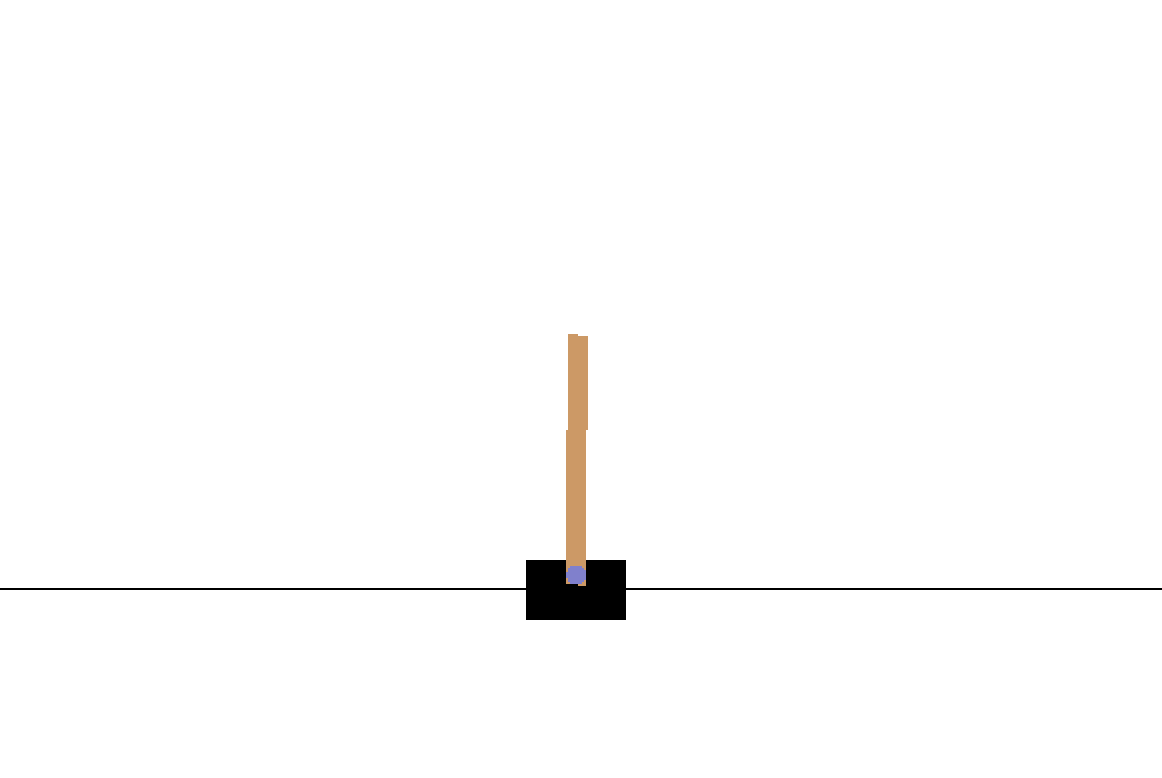
\includegraphics[scale=0.5]{include/cartpole.png}
    \caption{How the CartPole enviroment looks like}
    \label{fig:layers}
\end{figure}
the game ends when the pole is more than 15 degrees from vertical or the cart moves more than 2.4 units from the center.
\\ \\
By using OpenAI Gym the information needed for testing our algorithms is easy to collect. In all OpenAI Gym environments there exists a \textit{action space} with consist of the actions available in the environment, in CartPole there are only two actions \texttt{[moving left, moving right]}. 

In all environments it's posible to simulate a action, which is called a \textit{step} in OpenAI Gym. By performing an action the environment return a \textit{observation space}, \textit{reward} and \textit{done}. The observation space which in the theory section will be referred to as state, the observation space consist of information about the environment. In the CartPole environment the observation space consists of four elements \texttt{[position of cart, velocity of cart, angle of pole, rotation rate of pole]}. The reward is the reward achieved by taking the previous action, in the CartPole problem we achieve a reward of +1 for every action performed that not end the game. Done is just a signal which indicate whether the game is done or not.

We are also using the Atari environment, here are some example of what these look like,
\begin{figure}[H]
    \begin{subfigure}[b]{.5\textwidth}
        \centering
        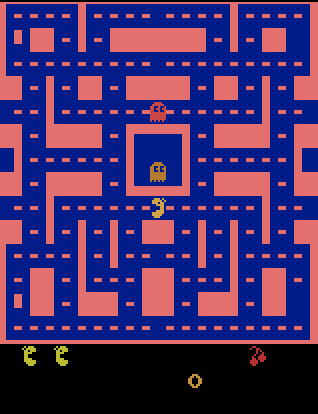
\includegraphics[scale=0.75]{include/pacman.png}
        \caption{Pacman environment}
    \end{subfigure}
    \begin{subfigure}[b]{.5\textwidth}
        \centering
        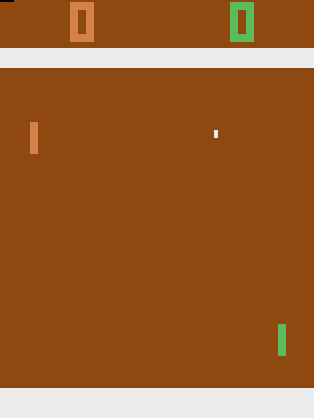
\includegraphics[scale=0.75]{include/pong.png}
        \caption{Pong environment}
    \end{subfigure}
    \vskip\baselineskip
    \begin{subfigure}[b]{.5\textwidth}
        \centering
        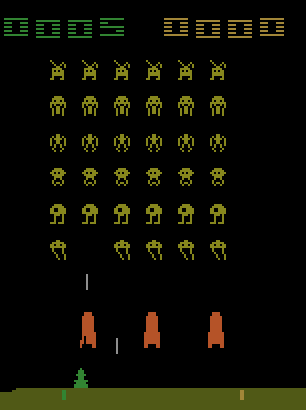
\includegraphics[scale=0.75]{include/space.png}
        \caption{Space invaders environment}
    \end{subfigure}
    \begin{subfigure}[b]{.5\textwidth}
        \centering
        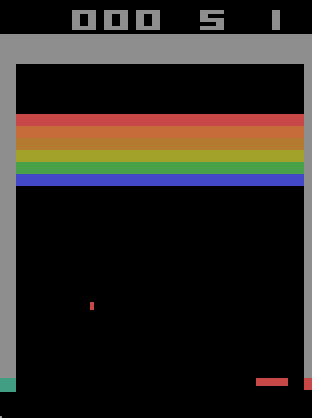
\includegraphics[scale=0.75]{include/breakout.png}
        \caption{Breakout environment}
    \end{subfigure}
    \caption{Four Atari environments}
    \label{fig:Atari_env}
\end{figure}
\end{document}
